\documentclass[11pt]{article}
\usepackage[margin=1in]{geometry}
\usepackage[T1]{fontenc}
\usepackage{lmodern}
\usepackage{amsmath,amssymb}
\usepackage{booktabs}
\usepackage{siunitx}
\usepackage{graphicx}
\usepackage{xcolor}
\usepackage[numbers,sort&compress]{natbib}
\usepackage{hyperref}
\usepackage{cleveref}
\hypersetup{colorlinks=true,linkcolor=blue!50!black,citecolor=blue!50!black,urlcolor=blue!50!black}

% GENERATED by figures/make_figures.py from results/summary.json -- do not edit.
\newcommand{\gpuName}{NVIDIA GeForce RTX 3070 Laptop GPU}
\newcommand{\nWorkloads}{9}
\newcommand{\copyBW}{361}
\newcommand{\specBW}{448}
\newcommand{\fmaPeak}{15.5}
\newcommand{\philoxRate}{112.6}
\newcommand{\LbmTwoDslPct}{100}
\newcommand{\LbmTwoDslBackend}{Numba-CUDA}
\newcommand{\LbmTwoCompilePct}{100}
\newcommand{\LbmTwoCompileBackend}{torch.compile}
\newcommand{\LbmTwoCudaPct}{100}
\newcommand{\LbmTwoCudaBackend}{CUDA C}
\newcommand{\LbmTwoDslOverCuda}{100}
\newcommand{\LbmTwoCpPct}{99}
\newcommand{\LbmTwoCpCode}{FluidX3D}
\newcommand{\LbmTwoDslOverCp}{1.02}
\newcommand{\LbmTwoCudaOverCp}{1.02}
\newcommand{\LbmThreeDslPct}{100}
\newcommand{\LbmThreeDslBackend}{Numba-CUDA}
\newcommand{\LbmThreeCompilePct}{81}
\newcommand{\LbmThreeCompileBackend}{torch.compile}
\newcommand{\LbmThreeCudaPct}{99}
\newcommand{\LbmThreeCudaBackend}{CUDA C}
\newcommand{\LbmThreeDslOverCuda}{100}
\newcommand{\LbmThreeCpPct}{99}
\newcommand{\LbmThreeCpCode}{FluidX3D}
\newcommand{\LbmThreeDslOverCp}{1.01}
\newcommand{\LbmThreeCudaOverCp}{1.00}
\newcommand{\HeatTwoDslPct}{100}
\newcommand{\HeatTwoDslBackend}{Triton}
\newcommand{\HeatTwoCompilePct}{101}
\newcommand{\HeatTwoCompileBackend}{torch.compile}
\newcommand{\HeatTwoCudaPct}{97}
\newcommand{\HeatTwoCudaBackend}{CUDA C}
\newcommand{\HeatTwoDslOverCuda}{103}
\newcommand{\HeatTwoCpPct}{99}
\newcommand{\HeatTwoCpCode}{pystencils}
\newcommand{\HeatTwoDslOverCp}{1.01}
\newcommand{\HeatTwoCudaOverCp}{0.98}
\newcommand{\HeatThreeDslPct}{91}
\newcommand{\HeatThreeDslBackend}{Numba-CUDA}
\newcommand{\HeatThreeCompilePct}{58}
\newcommand{\HeatThreeCompileBackend}{torch.compile}
\newcommand{\HeatThreeCudaPct}{89}
\newcommand{\HeatThreeCudaBackend}{CUDA C}
\newcommand{\HeatThreeDslOverCuda}{102}
\newcommand{\HeatThreeCpPct}{73}
\newcommand{\HeatThreeCpCode}{pystencils}
\newcommand{\HeatThreeDslOverCp}{1.25}
\newcommand{\HeatThreeCudaOverCp}{1.22}
\newcommand{\NbodyDslPct}{52}
\newcommand{\NbodyDslBackend}{Warp}
\newcommand{\NbodyCompilePct}{11}
\newcommand{\NbodyCompileBackend}{torch.compile}
\newcommand{\NbodyCudaPct}{54}
\newcommand{\NbodyCudaBackend}{CUDA C}
\newcommand{\NbodyDslOverCuda}{97}
\newcommand{\NbodyCpPct}{47}
\newcommand{\NbodyCpCode}{CUDA Samples nbody}
\newcommand{\NbodyDslOverCp}{1.10}
\newcommand{\NbodyCudaOverCp}{1.13}
\newcommand{\MdDslPct}{41}
\newcommand{\MdDslBackend}{Triton}
\newcommand{\MdCompilePct}{5}
\newcommand{\MdCompileBackend}{torch.compile}
\newcommand{\MdCudaPct}{45}
\newcommand{\MdCudaBackend}{CUDA C}
\newcommand{\MdDslOverCuda}{90}
\newcommand{\MdCpPct}{35}
\newcommand{\MdCpCode}{HOOMD-blue}
\newcommand{\MdDslOverCp}{1.17}
\newcommand{\MdCudaOverCp}{1.29}
\newcommand{\SpecTwoDslPct}{76}
\newcommand{\SpecTwoDslBackend}{Triton}
\newcommand{\SpecTwoCompilePct}{69}
\newcommand{\SpecTwoCompileBackend}{torch.compile}
\newcommand{\SpecTwoCudaPct}{99}
\newcommand{\SpecTwoCudaBackend}{CUDA C}
\newcommand{\SpecTwoDslOverCuda}{77}
\newcommand{\SpecTwoCpPct}{52}
\newcommand{\SpecTwoCpCode}{JAX-CFD}
\newcommand{\SpecTwoDslOverCp}{1.47}
\newcommand{\SpecTwoCudaOverCp}{1.91}
\newcommand{\SpecThreeDslPct}{80}
\newcommand{\SpecThreeDslBackend}{Warp}
\newcommand{\SpecThreeCompilePct}{64}
\newcommand{\SpecThreeCompileBackend}{torch.compile}
\newcommand{\SpecThreeCudaPct}{102}
\newcommand{\SpecThreeCudaBackend}{CUDA C}
\newcommand{\SpecThreeDslOverCuda}{78}
\newcommand{\IsingDslPct}{38}
\newcommand{\IsingDslBackend}{Warp}
\newcommand{\IsingCompilePct}{8}
\newcommand{\IsingCompileBackend}{torch.compile}
\newcommand{\IsingCudaPct}{42}
\newcommand{\IsingCudaBackend}{CUDA C}
\newcommand{\IsingDslOverCuda}{91}
\newcommand{\IsingCpPct}{29}
\newcommand{\IsingCpCode}{NVIDIA ising-gpu}
\newcommand{\IsingDslOverCp}{1.34}
\newcommand{\IsingCudaOverCp}{1.48}
\newcommand{\tbTwoOursX}{3.62}
\newcommand{\tbTwoOursK}{8}
\newcommand{\tbTwoAnX}{5.24}
\newcommand{\tbTwoAnK}{13}
\newcommand{\tbThreeOursX}{2.09}
\newcommand{\tbThreeOursK}{3}
\newcommand{\tbThreeAnX}{1.59}
\newcommand{\tbThreeAnK}{4}
\newcommand{\dslOverCudaMin}{77}
\newcommand{\dslOverCudaMax}{103}
\newcommand{\dslOverCudaMedian}{97}
\newcommand{\summaryRows}{LBM D2Q9 & memory & 100 & 100 (Numba-CUDA) & 100 & FluidX3D 99; Lettuce 27 \\
LBM D3Q19 & memory & 81 & 100 (Numba-CUDA) & 99 & FluidX3D 99; Lettuce 14 \\
heat 2D & memory & 101 & 100 (Triton) & 97 & pystencils 99 \\
heat 3D & memory & 58 & 91 (Numba-CUDA) & 89 & pystencils 73 \\
N-body & compute & 11 & 52 (Warp) & 54 & CUDA Samples nbody 47 \\
LJ MD & memory & 5 & 41 (Triton) & 45 & HOOMD-blue 35; LAMMPS 12 \\
spectral 2D & FFT & 69 & 76 (Triton) & 99 & JAX-CFD 52 \\
spectral 3D & FFT & 64 & 80 (Warp) & 102 & -- \\
Ising 2D & memory/RNG & 8 & 38 (Warp) & 42 & NVIDIA ising-gpu 29 \\}


\title{Python at the roofline:\\
nine GPU workloads against hand-written CUDA and established codes}
\author{Walid Hemati\\Independent researcher}
\date{}

\begin{document}
\maketitle

\begin{abstract}
We test one claim across six simulation codes: GPU kernels written and launched from Python reach
the same \emph{hardware efficiency} as hand-written CUDA and as established high-performance
codes. The six open-source packages cover lattice-Boltzmann flow (D2Q9 and D3Q19), explicit
stencils (2D and 3D), direct-summation $N$-body gravity, Lennard-Jones molecular dynamics,
pseudo-spectral Navier--Stokes (2D and 3D) and Ising Monte Carlo, nine workloads in all. Each is
implemented along the same ladder (NumPy, PyTorch, \texttt{torch.compile}, the Python GPU
languages Triton, NVIDIA Warp and Numba-CUDA, and hand-written CUDA~C compiled at run time), validated
against analytic or reference results, and measured on one \gpuName{} against a ceiling measured
on that GPU: copy bandwidth (\SI{\copyBW}{GB/s}) for memory-bound kernels, FP32 FMA throughput
(\SI{\fmaPeak}{TFLOPS}) for $N$-body, cuFFT for spectral methods and copy bandwidth plus Philox
throughput for Ising. Across the nine workloads the best kernel written entirely in a Python GPU
language reaches \dslOverCudaMin--\dslOverCudaMax\,\% (median \dslOverCudaMedian\,\%) of the
efficiency of our hand-written CUDA~C. We also ran established codes on the same GPU: FluidX3D,
Lettuce, pystencils, AN5D, the CUDA Samples \texttt{nbody}, LAMMPS, HOOMD-blue, JAX-CFD,
spectralDNS, Dedalus and NVIDIA's \texttt{ising-gpu}. At the levels compared, the Python-launched kernels match or exceed the best of them on all
nine workloads; the exception is the temporal-blocking rung of the 2D stencil, where the code
generator AN5D is ahead. Where Python falls short of CUDA~C, the
missing piece is a schedule (a marching order, a fused transform plan), not the language.
\end{abstract}

\section{Introduction}

Scientific GPU codes are usually written in CUDA~C/C++ or Fortran, and Python is used to drive
them. Python-hosted GPU languages (Triton~\citep{tillet2019triton}, NVIDIA
Warp~\citep{macklin2022warp}, Numba-CUDA~\citep{lam2015numba}) and compilers for array code
(\texttt{torch.compile}~\citep{ansel2024pytorch2}) now let the kernel itself be written in Python.
Whether such kernels are competitive is often argued with single benchmarks on different
hardware. We instead measure every kernel as a fraction of a roofline~\citep{williams2009roofline}
measured on the same GPU, for nine workloads from six independent packages, and we run
established codes for the same workloads on that GPU.

Contributions:
\begin{itemize}
  \item Six open-source packages (\texttt{pylbm}, \texttt{pyheat3d}, \texttt{pygravity},
        \texttt{pymd}, \texttt{pyspectral}, \texttt{pyising}), each with the same backend
        ladder, a NumPy oracle, physics validation and a benchmark that writes every number of
        its paper from a results file.
  \item A common measurement protocol: one GPU, measured ceilings, minimal traffic models,
        serial runs on an idle GPU, medians of five repeats.
  \item Same-GPU head-to-heads with eleven established codes, with each counterpart checked
        to solve the same problem as ours.
  \item A cross-workload comparison (\cref{fig:eff,tab:summary}) of where Python GPU languages
        reach hand-written CUDA~C, where \texttt{torch.compile} suffices, and where neither does.
\end{itemize}
Each package has its own paper with the full method, validation and results; this paper
summarises them and draws the common conclusions.

\section{Method}

\paragraph{Hardware and ceilings.} All measurements use one \gpuName{} (GA104, 40 SMs, 8\,GB
GDDR6, \SI{\specBW}{GB/s} specification bandwidth). The device-to-device copy bandwidth measured
with 1\,GiB buffers is \SI{\copyBW}{GB/s}; an FMA-chain microbenchmark gives
\SI{\fmaPeak}{TFLOPS} in FP32; the Philox4x32-10 generator~\citep{Salmon2011} used for Monte Carlo
runs at \philoxRate{} calls per ns; cuFFT~\citep{cufft} times are measured per transform size.

\paragraph{Rooflines.} Each workload uses the ceiling that bounds it (\cref{tab:summary}). For
memory-bound kernels the bound is copy bandwidth divided by the \emph{minimal} DRAM traffic of
one update (e.g.\ $2Q$ populations for lattice Boltzmann, one read and one write per stencil
point, read-own/read-neighbour/write-own per spin). The minimal model never inflates effective
bandwidth; kernels slightly above 100\,\% move a little less than the copy kernel's traffic per
byte, or hit in the L2 cache. For $N$-body the bound is the FMA peak at 20 flops per interaction.
For pseudo-spectral DNS it is the time of the step's FFTs as standalone cuFFT calls plus the
minimal traffic of the pointwise work. For Ising it is the smaller of the bandwidth bound and
the Philox bound, with the random numbers a spin update actually needs.

\paragraph{The ladder.} Every package implements the same algorithm in: NumPy (the correctness
oracle), PyTorch eager~\citep{paszke2019pytorch}, \texttt{torch.compile} (the same tensor code,
compiled by Inductor into Triton), hand-written kernels in Triton, Warp and Numba-CUDA (``Python
GPU languages'' below), and hand-written CUDA~C compiled at run time by NVRTC through
CuPy~\citep{okuta2017cupy} and launched from Python. All backends share one interface and are
checked against the NumPy oracle; most packages reproduce it bit for bit.

\paragraph{Measurement.} Benchmarks warm up (including JIT compilation and autotuning),
synchronise the device around timed regions, run each timed repeat for at least \SI{0.5}{s} and
report the median of five repeats. The final numbers come from one serial run per package on an
otherwise idle GPU. For each implementation class we report the best variant at the largest
problem size it reached: small grids can exceed the DRAM roofline because part of the working
set stays in the 4\,MB L2 cache.

\paragraph{Counterparts.} For each workload we chose established codes that solve the same
problem and could be built here, built them from pinned commits without changing their
algorithms, and checked that they reproduce our results before timing them. Where the
counterpart runner applied our traffic model or ceiling directly (lattice Boltzmann, stencils,
$N$-body) we quote that percentage. Otherwise (MD, spectral, Ising) we divide the counterpart's
throughput by our CUDA~C throughput measured in the same session at the same problem size, and
multiply by our kernel's roofline fraction. The details, including every build patch, are in the
package papers.

\section{Results}

\begin{figure}[t]
\centering
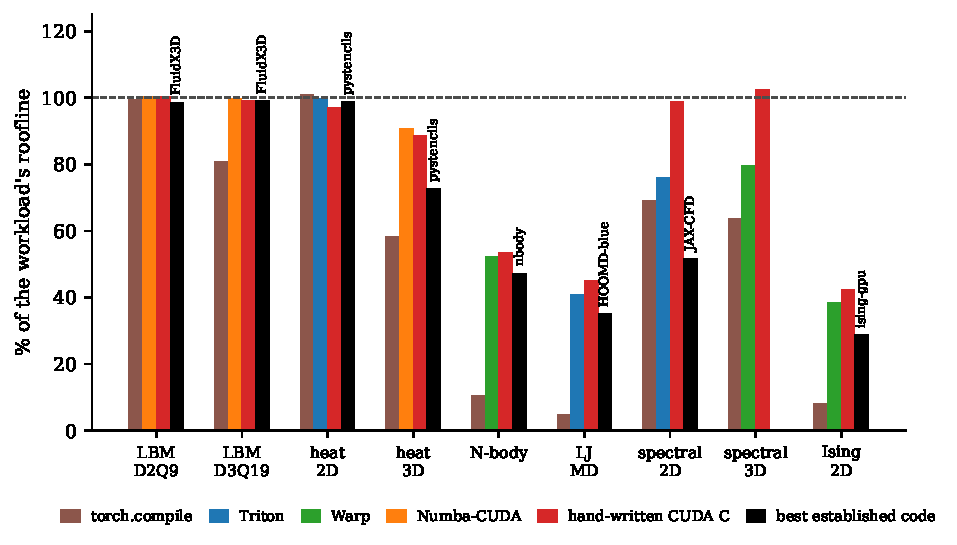
\includegraphics[width=\linewidth]{../figures/efficiency.pdf}
\caption{Best implementation of each class as a percentage of the workload's roofline:
\texttt{torch.compile}, the best kernel written in a Python GPU language (bar colour: Triton,
Warp or Numba), hand-written CUDA~C launched from Python, and the best established code run on
the same GPU. Dashed: the roofline.}
\label{fig:eff}
\end{figure}

\begin{table}[t]
\centering\footnotesize\setlength{\tabcolsep}{4pt}
\caption{Percent of each workload's roofline at the largest problem size (\cref{fig:eff}). The
last column lists the best one or two established codes.}
\label{tab:summary}
\begin{tabular}{llrlrl}
\toprule
workload & bound & compile & Python GPU lang. & CUDA C & established code \\
\midrule
\summaryRows
\bottomrule
\end{tabular}
\end{table}

\Cref{fig:eff,tab:summary} summarise the nine workloads.

\paragraph{Lattice Boltzmann.} Fused stream--collide kernels in all three Python languages run at
the copy bandwidth: \LbmTwoDslPct\,\% (D2Q9) and \LbmThreeDslPct\,\% (D3Q19), the same as CUDA~C
(\LbmTwoCudaPct\,\%, \LbmThreeCudaPct\,\%) and as the hand-optimised OpenCL code
FluidX3D~\citep{lehmann2022} (\LbmTwoCpPct\,\%, \LbmThreeCpPct\,\%). \texttt{torch.compile}
reaches the roofline in 2D (\LbmTwoCompilePct\,\%) but not in 3D (\LbmThreeCompilePct\,\%). The
PyTorch framework Lettuce~\citep{bedrunka2021} with its native kernels is far below.

\paragraph{Stencils.} Single-step heat-equation kernels reach \HeatTwoDslPct\,\% (2D) and
\HeatThreeDslPct\,\% (3D) in a Python language, against \HeatTwoCudaPct\,\% and \HeatThreeCudaPct\,\%
for CUDA~C and \HeatTwoCpPct\,\% and \HeatThreeCpPct\,\% for pystencils~\citep{bauer2019pystencils}.
In 3D the difference is the schedule: kernels that march along $z$ reach the bound, one thread
per point (pystencils, \texttt{torch.compile} at \HeatThreeCompilePct\,\%) does not. Temporal
blocking raises the per-update roofline: our CUDA~C kernels reach $\tbTwoOursX\times$ the
single-step roofline in 2D ($k=\tbTwoOursK$ fused steps) and $\tbThreeOursX\times$ in 3D
($k=\tbThreeOursK$); AN5D~\citep{matsumura2020an5d} reaches $\tbTwoAnX\times$ ($k=\tbTwoAnK$) and
$\tbThreeAnX\times$ ($k=\tbThreeAnK$). This rung is CUDA~C, because temporal blocking needs explicit
shared-memory schedules that Triton does not expose.

\paragraph{$N$-body.} The tiled force kernel reaches \NbodyDslPct\,\% of the FMA peak in
\NbodyDslBackend{} and \NbodyCudaPct\,\% in CUDA~C; the CUDA Samples \texttt{nbody}~\citep{nyland2007,
cudasamples} reaches \NbodyCpPct\,\% with fast math. Instruction counts explain the level: an
interaction needs more issue slots than its 20 nominal flops (see the \texttt{pygravity} paper).
\texttt{torch.compile} reaches \NbodyCompilePct\,\%.

\paragraph{Molecular dynamics.} With neighbour lists, the best Python-language kernel
(\MdDslBackend) reaches \MdDslPct\,\% of the bandwidth bound and CUDA~C \MdCudaPct\,\%, against
\MdCpPct\,\% for \MdCpCode~\citep{anderson2020hoomd} and less for LAMMPS~\citep{thompson2022lammps}
with its KOKKOS~\citep{trott2022kokkos} and GPU packages. The traffic model counts only the
minimal neighbour-list and position traffic, so these fractions are lower bounds.

\paragraph{Pseudo-spectral DNS.} The fused in-place CUDA~C kernels around batched cuFFT plans
reach the FFT roofline (\SpecTwoCudaPct\,\% in 2D, \SpecThreeCudaPct\,\% in 3D). The Python
languages reach \SpecTwoDslPct\,\% and \SpecThreeDslPct\,\%, \texttt{torch.compile}
\SpecTwoCompilePct\,\% and \SpecThreeCompilePct\,\%. JAX-CFD~\citep{dresdner2022learning} reaches
\SpecTwoCpPct\,\% of the same roofline in 2D; spectralDNS~\citep{mortensen2016high} (CPU) and the
GPU branch of Dedalus~\citep{burns2020dedalus} are compared in the \texttt{pyspectral} paper.

\paragraph{Ising Monte Carlo.} One-bit multi-spin coding reaches \IsingDslPct\,\% of the roofline
in \IsingDslBackend{} and \IsingCudaPct\,\% in CUDA~C; NVIDIA's \texttt{cuIsingModel}
\citep{Bisson2025,IsingGPURepo} reaches \IsingCpPct\,\% and the 4-bit code of
\citet{Romero2020} less. Neither code reaches the bandwidth bound; the work per spin, mostly
random-number generation, sets the level.

\section{Discussion}

\paragraph{Python GPU languages reach CUDA~C.} On every workload the best Triton, Warp or
Numba kernel is within a few percent of our CUDA~C, or ahead, except pseudo-spectral DNS
(\SpecTwoDslOverCuda\,\% and \SpecThreeDslOverCuda\,\% of the CUDA~C efficiency), molecular
dynamics (\MdDslOverCuda\,\%) and Ising (\IsingDslOverCuda\,\%). In the spectral codes the gap is
in the transforms: the CUDA~C path uses in-place batched cuFFT plans and fuses the pointwise work
around them, while the Python-language kernels call the library through higher-level
interfaces. In MD and Ising the kernels implement the same algorithm; the package papers attribute the
remaining differences to code generation (vector versus scalar loads, 64-bit index arithmetic,
unrolling), measured instruction by instruction for $N$-body and not profiled in depth for the
others.

\paragraph{\texttt{torch.compile} is enough for one fused loop.} When the whole step is a
pointwise expression over a regular grid (2D lattice Boltzmann, the 2D stencil),
\texttt{torch.compile} reaches the roofline with no kernel code at all. It falls short where
the efficient kernel needs a schedule that the tensor program does not express: marching through
$z$ in 3D, shared-memory tiling for $N$-body, neighbour-list gathers in MD, bit-sliced logic for
Ising.

\paragraph{Established codes.} On this GPU the Python-launched kernels match or exceed the
best established code on all nine workloads of \cref{fig:eff}, and lose on one further rung,
deep temporal blocking in 2D. Several counterparts were tuned for other GPUs
(AN5D for P100/V100, \texttt{ising-gpu} on data-centre parts) and some run their own test case
(FluidX3D, Lettuce); the package papers state each difference. The one clear loss, AN5D's deep 2D
temporal blocking, is a comparison between hand-written and generated CUDA, not between Python
and C. We read the head-to-heads as evidence that the Python-launched kernels are not slow
reference implementations, not as rankings of those codes.

\paragraph{Threats to validity.} (i) One laptop GPU: clocks depend on temperature and power, and
absolute rates do not transfer; percentages of measured ceilings transfer better. (ii) Our
CUDA~C is compiled by NVRTC, not \texttt{nvcc} with tuned flags. (iii) Each roofline is a model;
the minimal traffic models make memory-bound fractions upper bounds on efficiency for the
kernels and lower bounds on the bandwidth they achieve. (iv) Counterparts were built from pinned
commits with minimal build patches and not retuned for this GPU. (v) The ``best variant'' of a
class is chosen after the fact from the measured runs.

\section{Conclusion}
Across nine GPU workloads, kernels written in Python GPU languages reach
\dslOverCudaMin--\dslOverCudaMax\,\% of the efficiency of hand-written CUDA~C on the same GPU,
and the best Python-launched kernels match or exceed the best established code on each of
them, with deep 2D temporal blocking as the one rung where a generated CUDA code is ahead. What
decided the result was always the algorithm and its schedule: minimal traffic, fused passes,
tiling, random bits per spin, FFT counts. Where those are expressed, Python reaches the
roofline.

\section*{Code availability}
All code is MIT-licensed at \url{https://github.com/walidhemati}: the repositories
\texttt{pylbm}, \texttt{pyheat3d}, \texttt{pygravity}, \texttt{pymd}, \texttt{pyspectral},
\texttt{pyising} and, for this summary, \texttt{pyhpc-overview}.
\texttt{collect.py} and \texttt{figures/make\_figures.py} regenerate every number here from the
packages' results files.

\bibliographystyle{unsrtnat}
\bibliography{references}

\end{document}
